
\phantomsection
\setstretch{1.5}
\justify
\fontsize{14}{16}\selectfont
\setlength{\parindent}{0pt}
\section*{V. Wyniki } 
\addcontentsline{toc}{chapter}{\textnormal{V. Wyniki }}
\fontsize{12}{14}\selectfont
% \vspace{\baselineskip} 

\hspace{1.5cm} Powstały kod, można uruchomić w interpreterze języka Python.
Domyślne środowisko to "\textit{Jupyter Notebook}" ze względu na występowanie plików w formacie 'ipynb', ale popularne edytory tekstu jak naprzykład "VS Code", albo IDE "\textit{PyCharm}" też potrafią obsługiwać tego typu pliki.

\hspace{1.5cm} Zgrupowano wykresy względem modeli. Każdy wykres przedstawia efektywność modelu względem wartości rzeczywistych.
Na osi rzędnych są wartości przewidziane, na odciętych prawdziwe.


\begin{figure}[ht]
\centering
\subfigure[Moduł sprężystości objętościowej]{%
    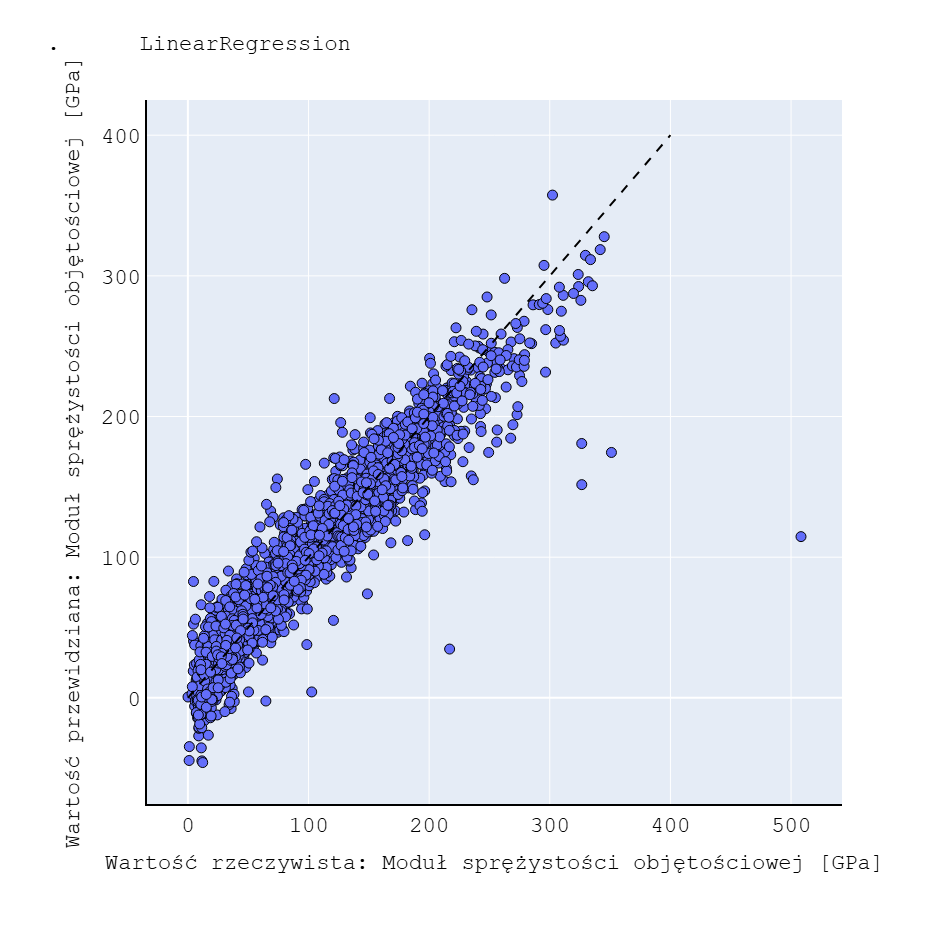
\includegraphics[width=0.48\textwidth]{images/figures/newplot (0).png}
}
\subfigure[Moduł sprężystości poprzecznej]{%
    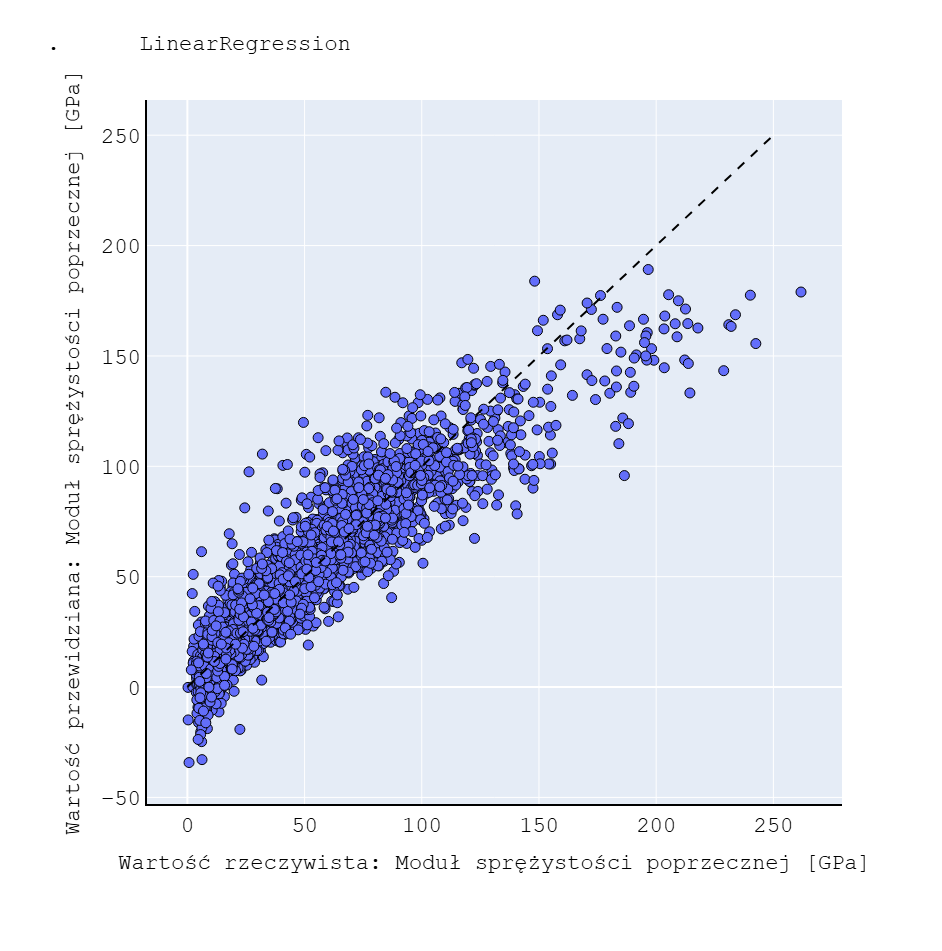
\includegraphics[width=0.48\textwidth]{images/figures/newplot (9).png}
}
\\
\subfigure[Współczynninik Anizotropii]{%
    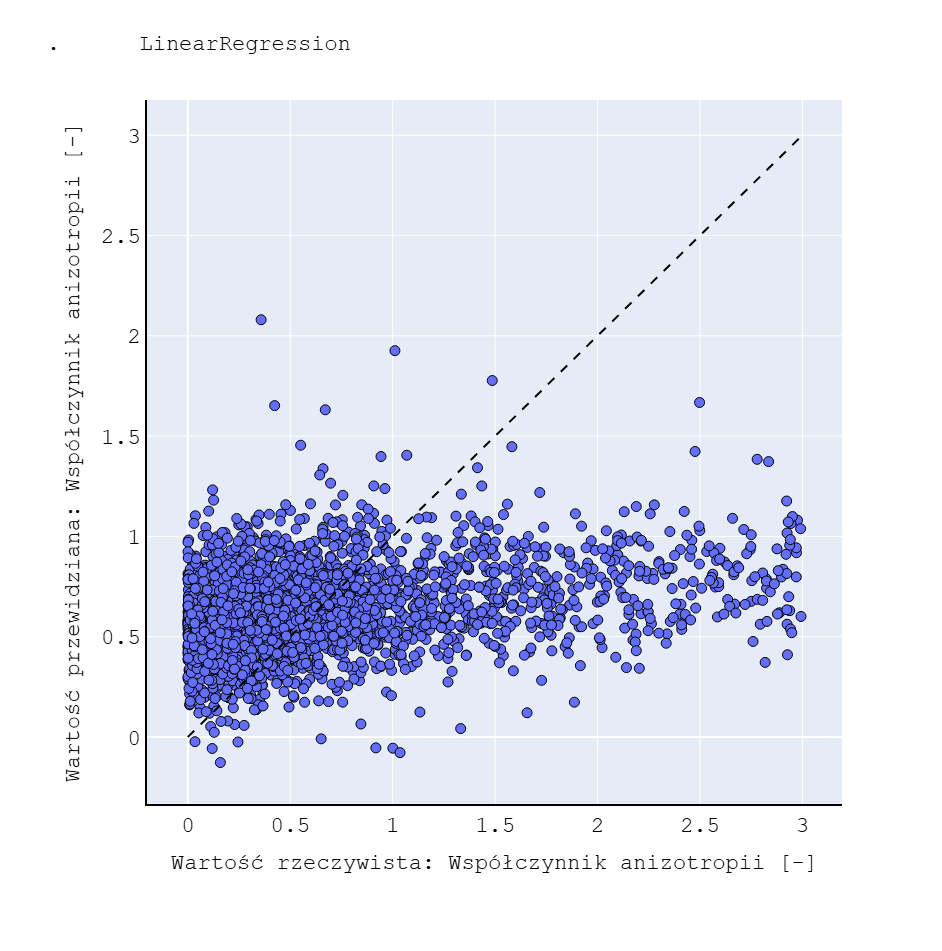
\includegraphics[width=0.48\textwidth]{images/figures/newplot (18).png}
}
\subfigure[Liczba Poisona]{%
    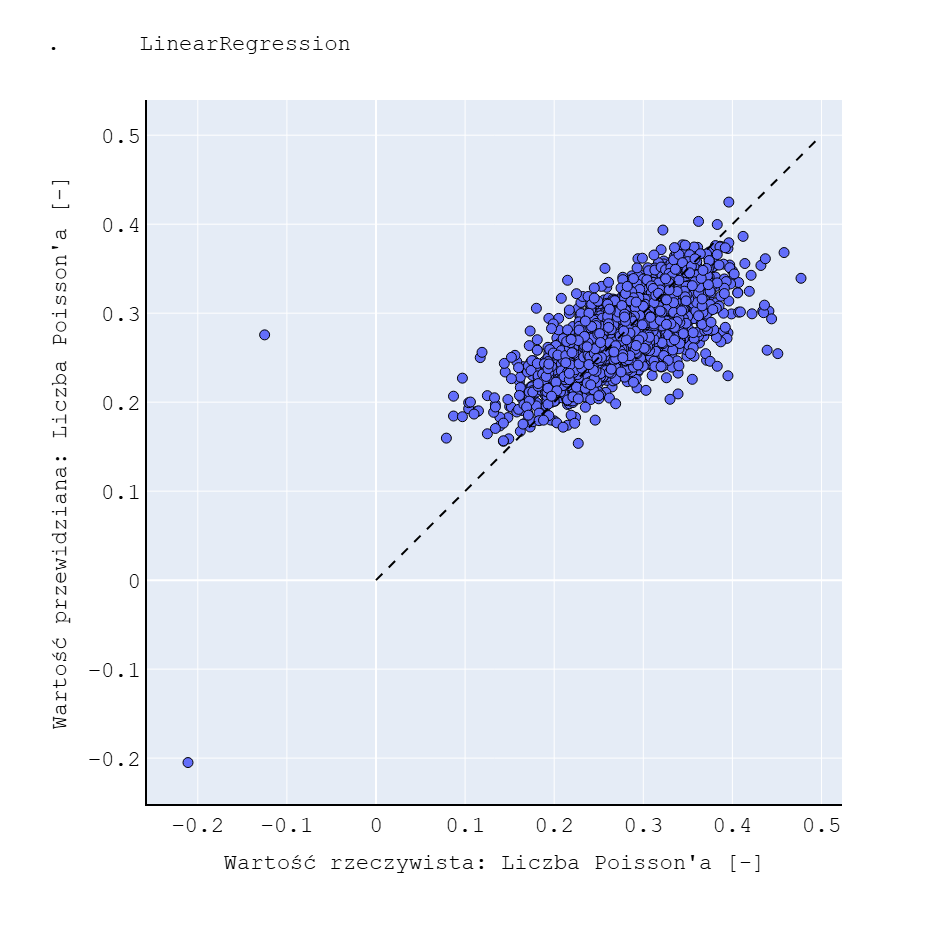
\includegraphics[width=0.48\textwidth]{images/figures/newplot (27).png}
}
\caption{Regresja Liniowa}
\end{figure}


\clearpage
\begin{figure}[ht]
\centering
\subfigure[Moduł sprężystości objętościowej]{%
    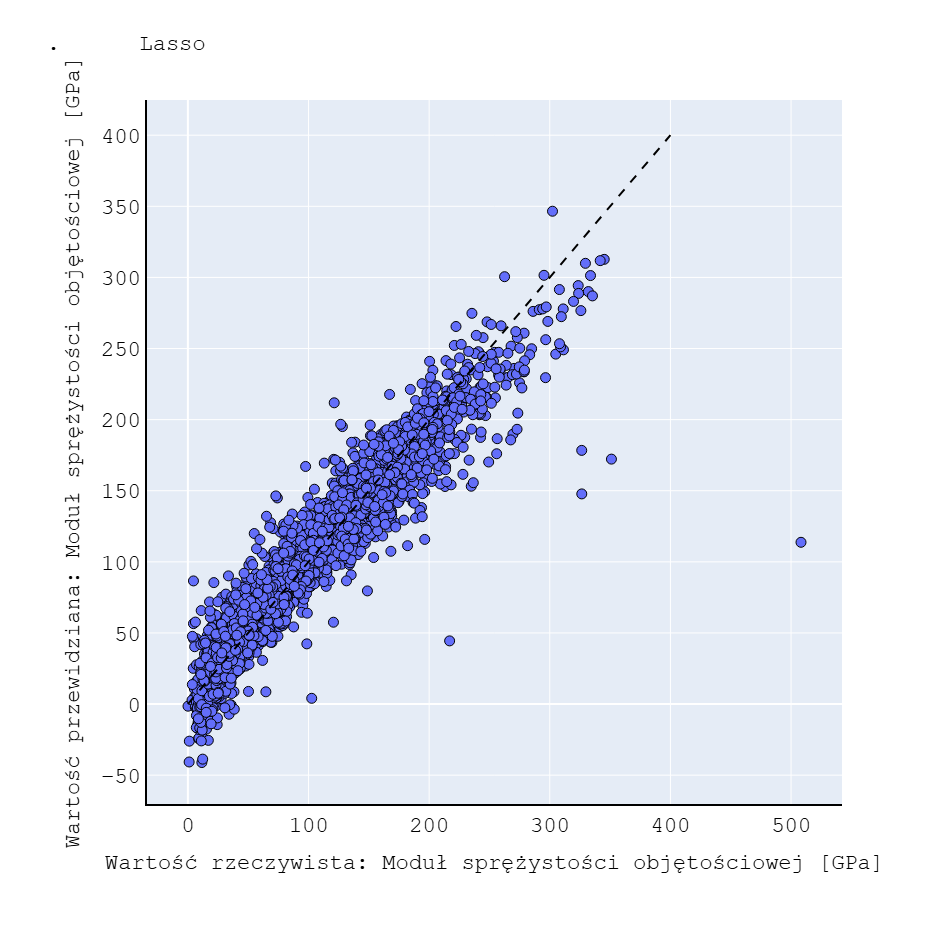
\includegraphics[width=0.48\textwidth]{images/figures/newplot (1).png}
}
\subfigure[Moduł sprężystości poprzecznej]{%
    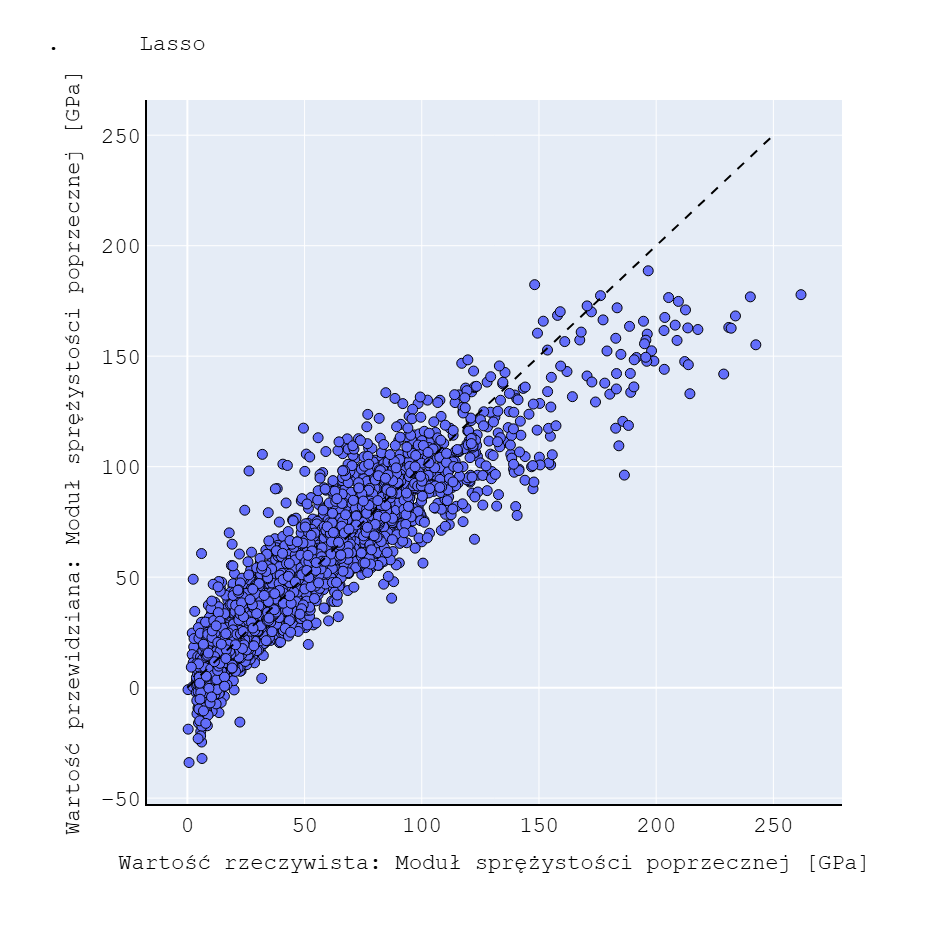
\includegraphics[width=0.48\textwidth]{images/figures/newplot (10).png}
}
\\
\subfigure[Współczynninik Anizotropii]{%
    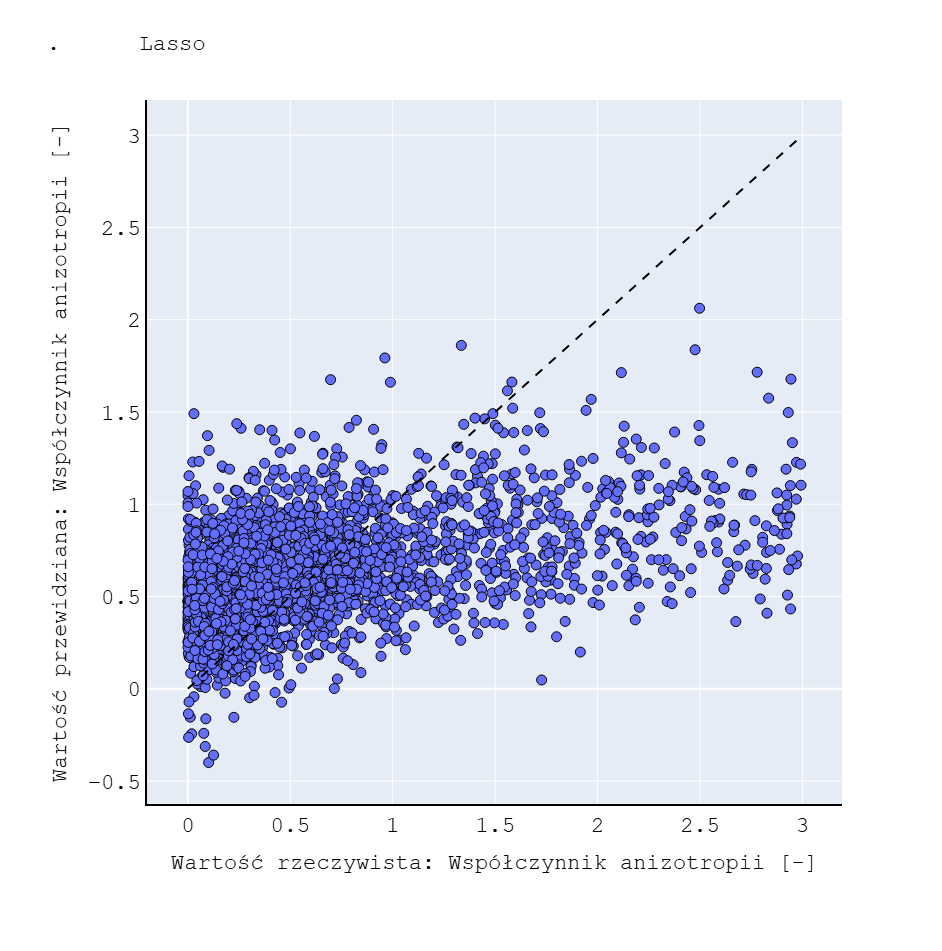
\includegraphics[width=0.48\textwidth]{images/figures/newplot (19).png}
}
\subfigure[Liczba Poisona]{%
    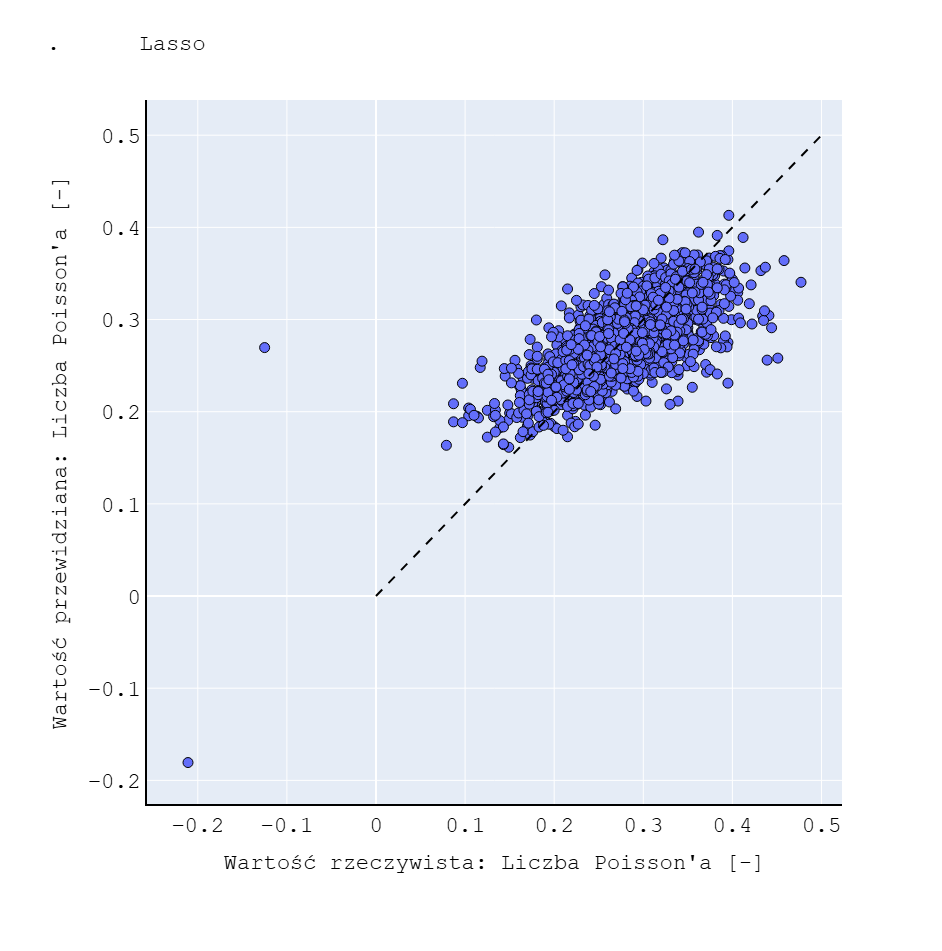
\includegraphics[width=0.48\textwidth]{images/figures/newplot (28).png}
}
\caption{Regresja Lasso}
\end{figure}


\clearpage
\begin{figure}[ht]
\centering
\subfigure[Moduł sprężystości objętościowej]{%
    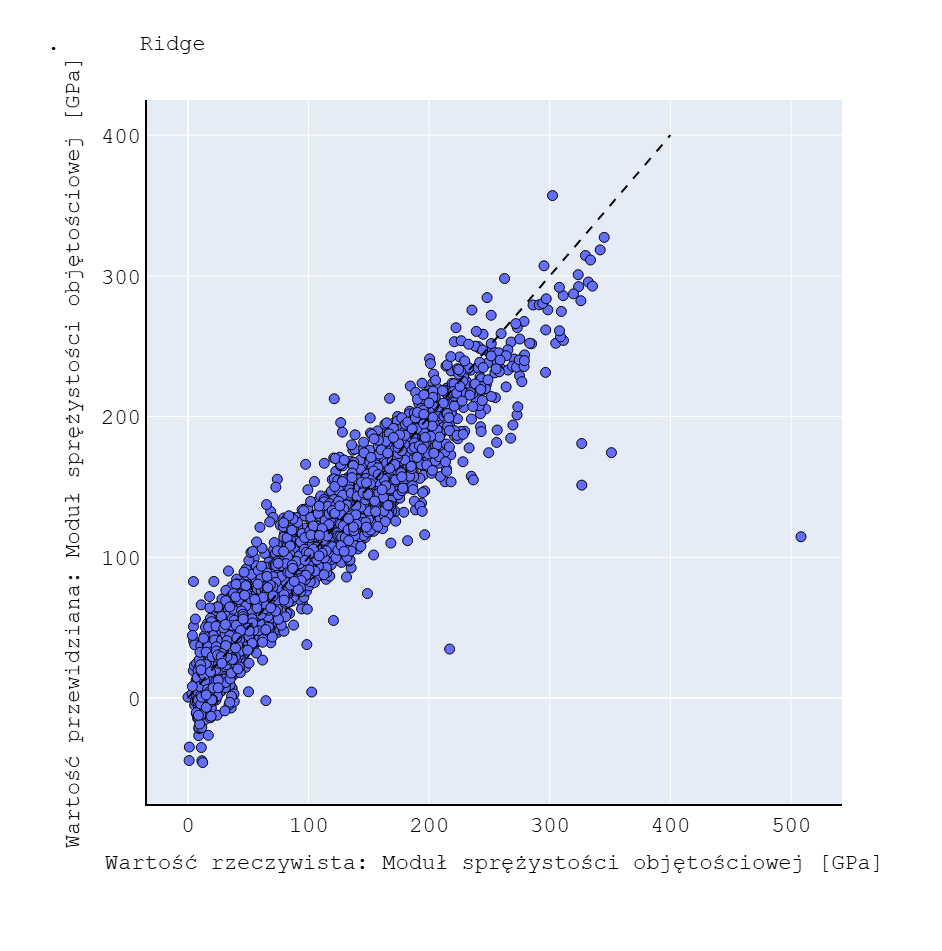
\includegraphics[width=0.48\textwidth]{images/figures/newplot (2).png}
}
\subfigure[Moduł sprężystości poprzecznej]{%
    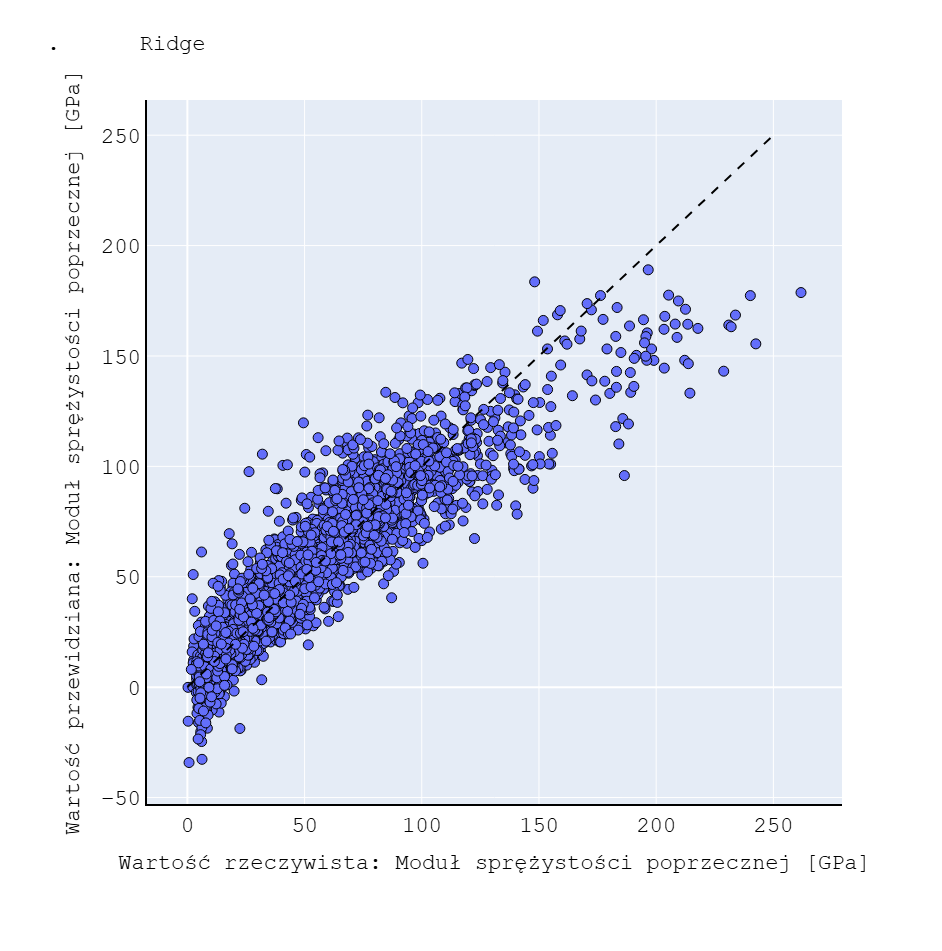
\includegraphics[width=0.48\textwidth]{images/figures/newplot (11).png}
}
\\
\subfigure[Współczynninik Anizotropii]{%
    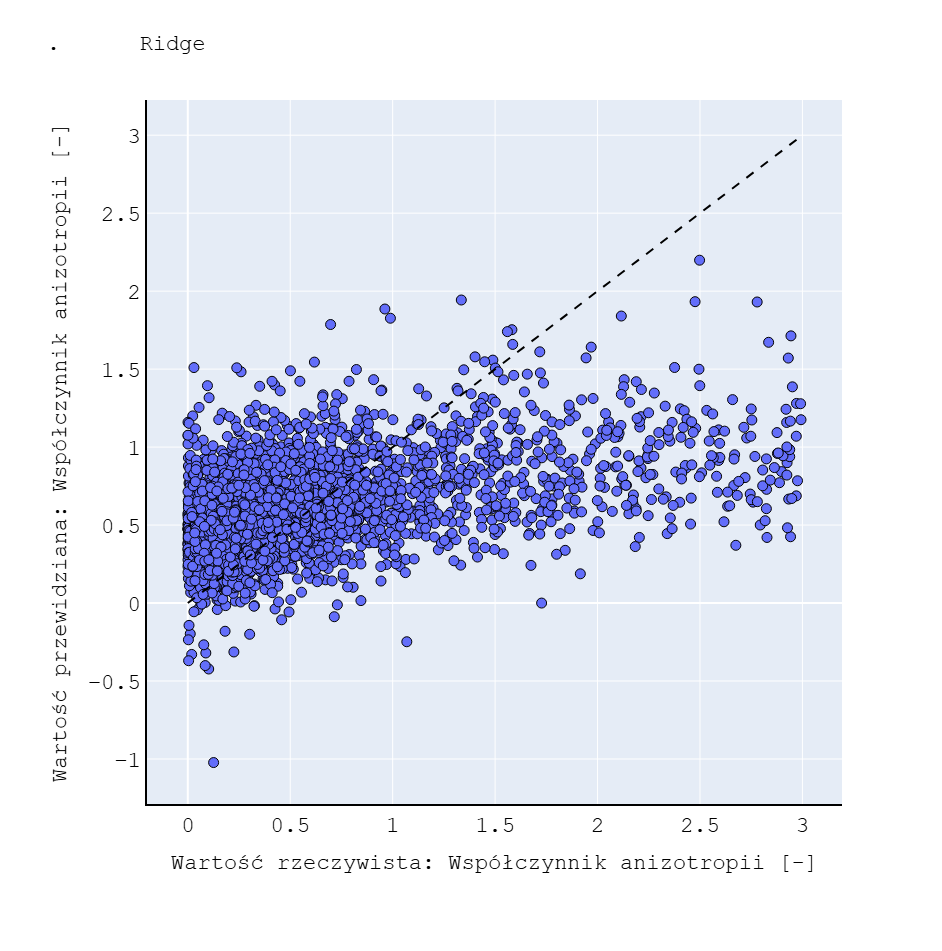
\includegraphics[width=0.48\textwidth]{images/figures/newplot (20).png}
}
\subfigure[Liczba Poisona]{%
    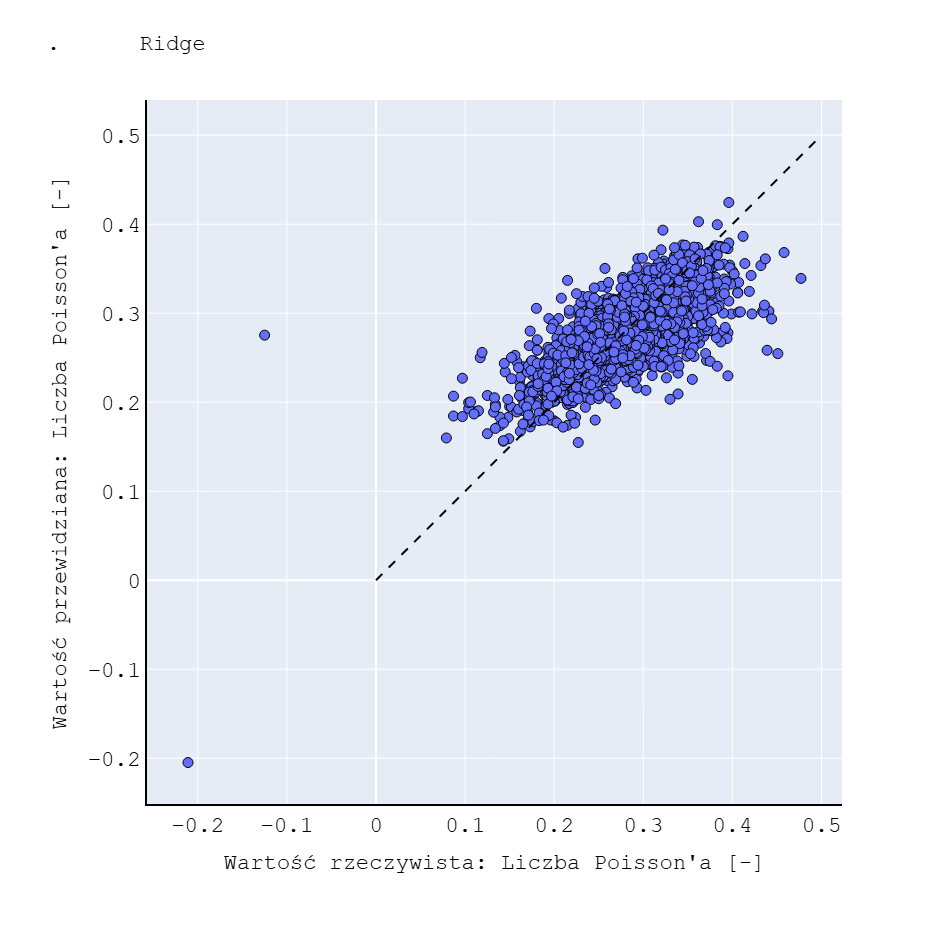
\includegraphics[width=0.48\textwidth]{images/figures/newplot (29).png}
}
\caption{Regresja Grzbietowa}
\end{figure}



\clearpage
\begin{figure}[ht]
\centering
\subfigure[Moduł sprężystości objętościowej]{%
    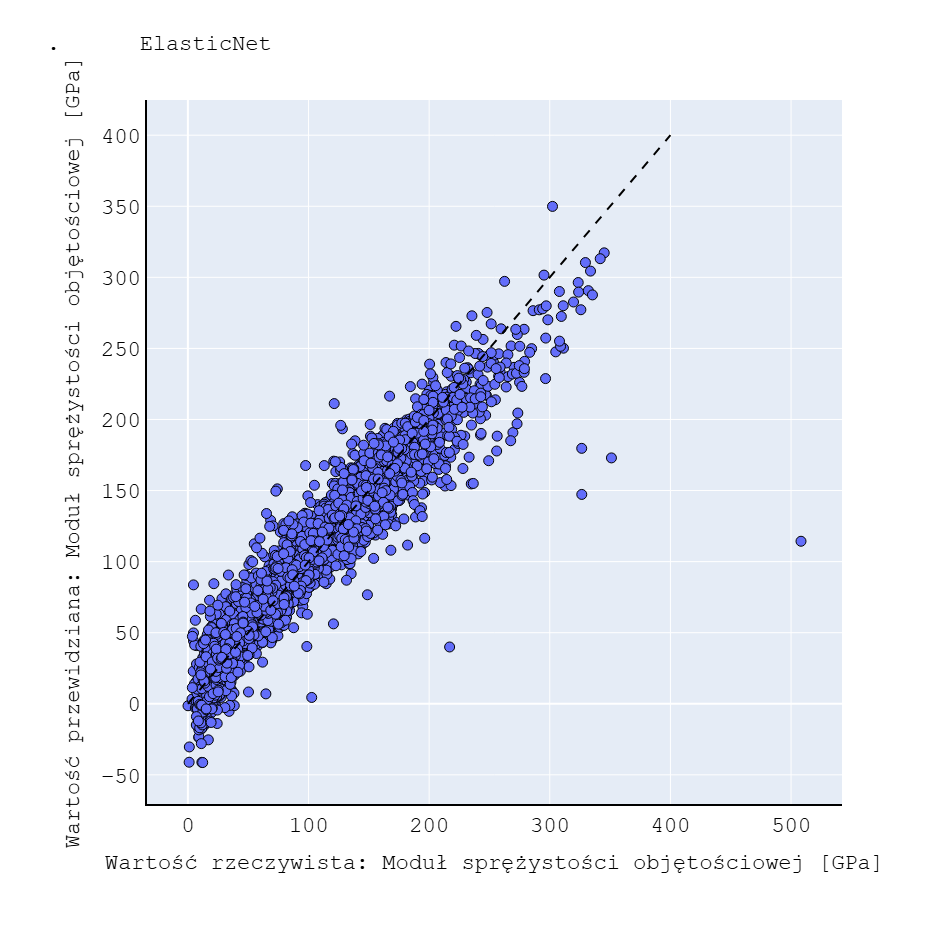
\includegraphics[width=0.48\textwidth]{images/figures/newplot (3).png}
}
\subfigure[Moduł sprężystości poprzecznej]{%
    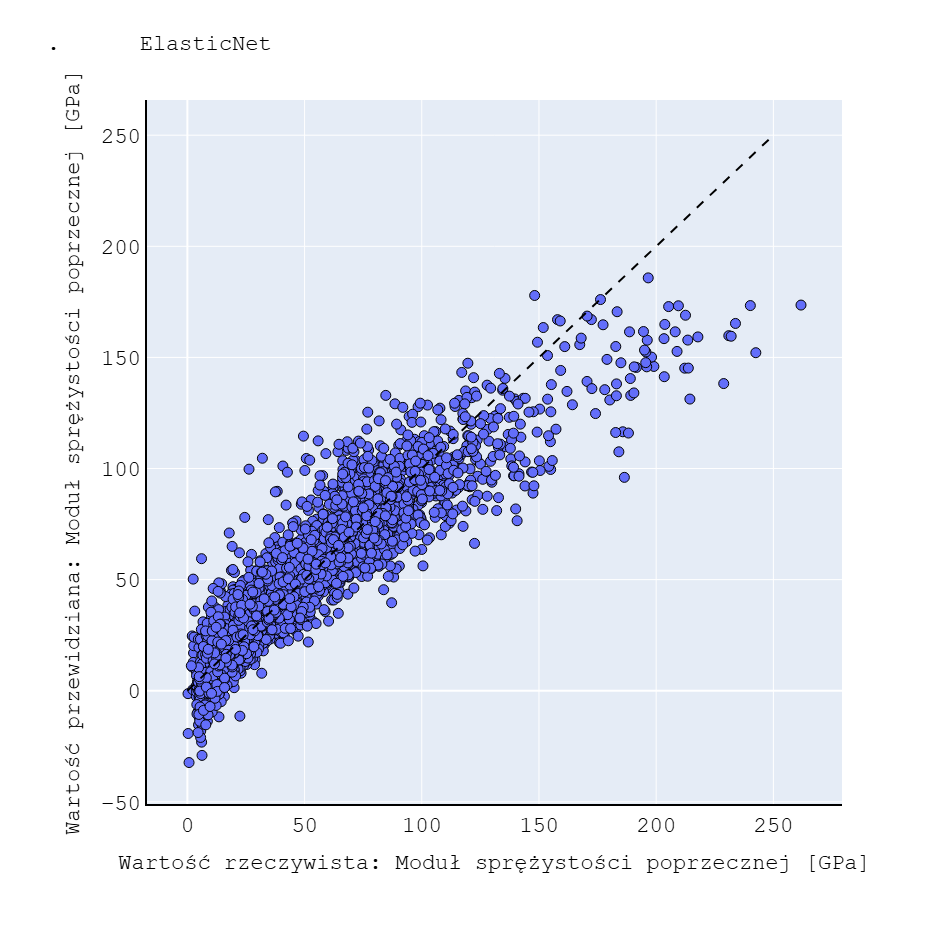
\includegraphics[width=0.48\textwidth]{images/figures/newplot (12).png}
}
\\
\subfigure[Współczynninik Anizotropii]{%
    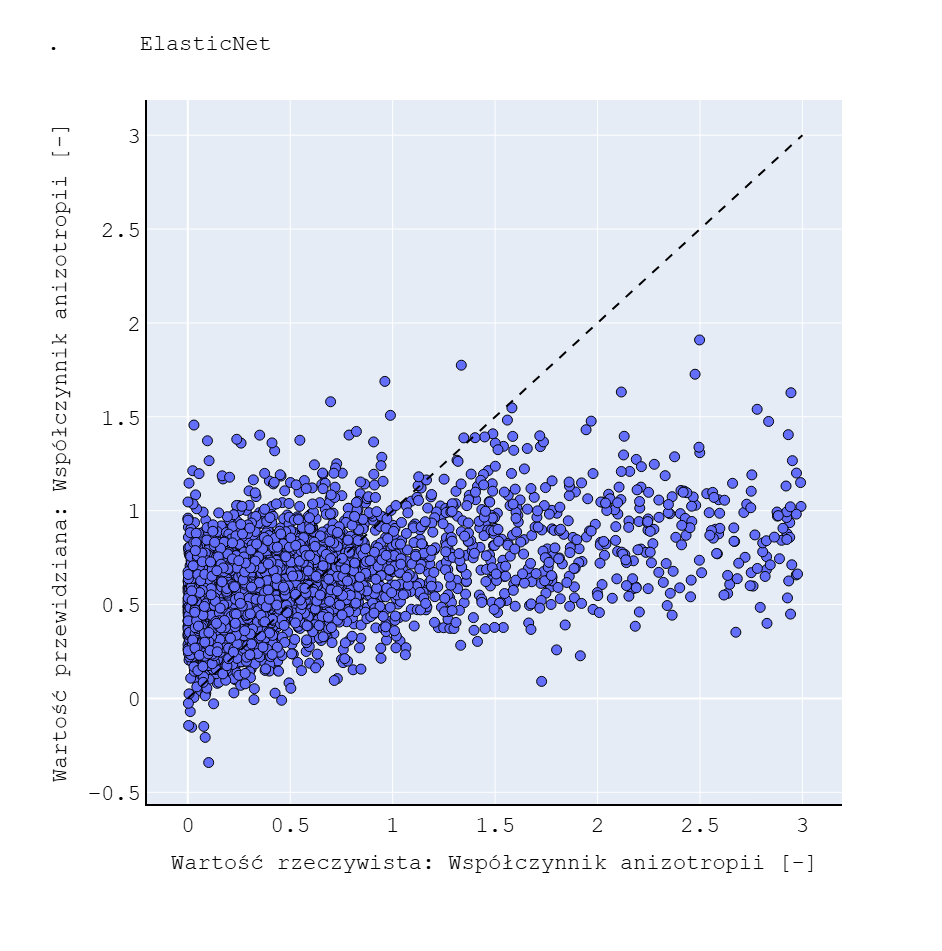
\includegraphics[width=0.48\textwidth]{images/figures/newplot (21).png}
}
\subfigure[Liczba Poisona]{%
    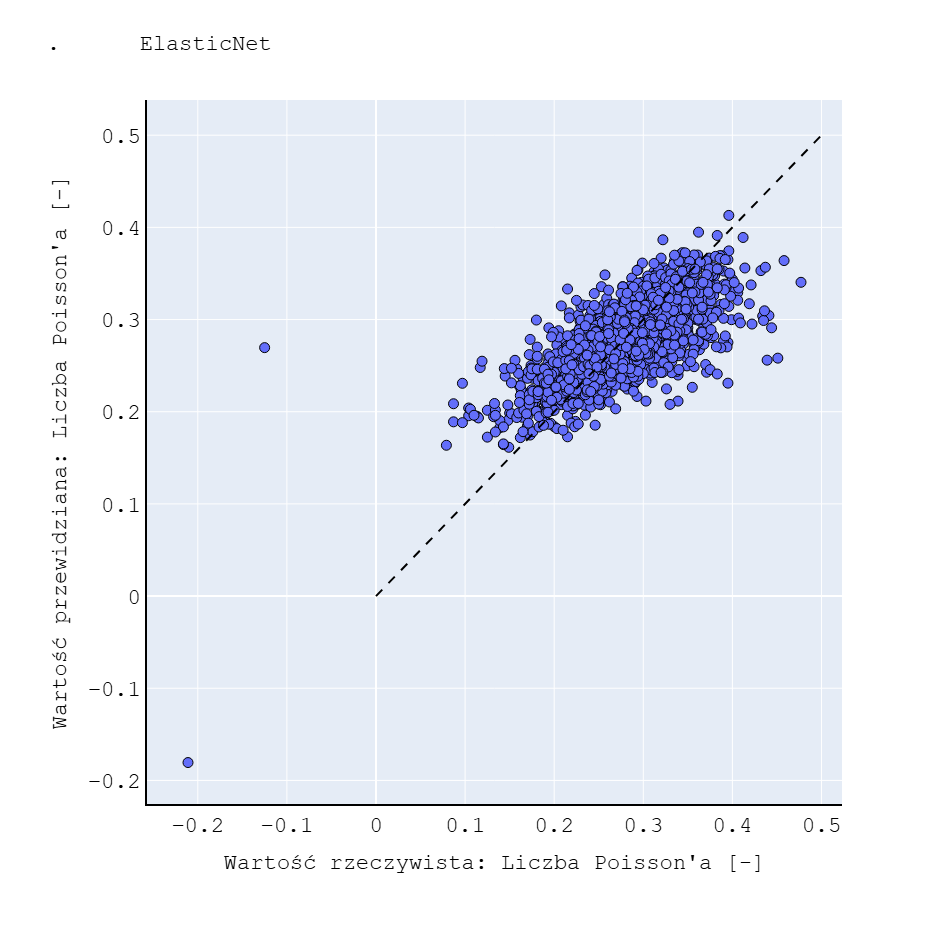
\includegraphics[width=0.48\textwidth]{images/figures/newplot (30).png}
}
\caption{Elastic Net}
\end{figure}



\clearpage
\begin{figure}[ht]
\centering
\subfigure[Moduł sprężystości objętościowej]{%
    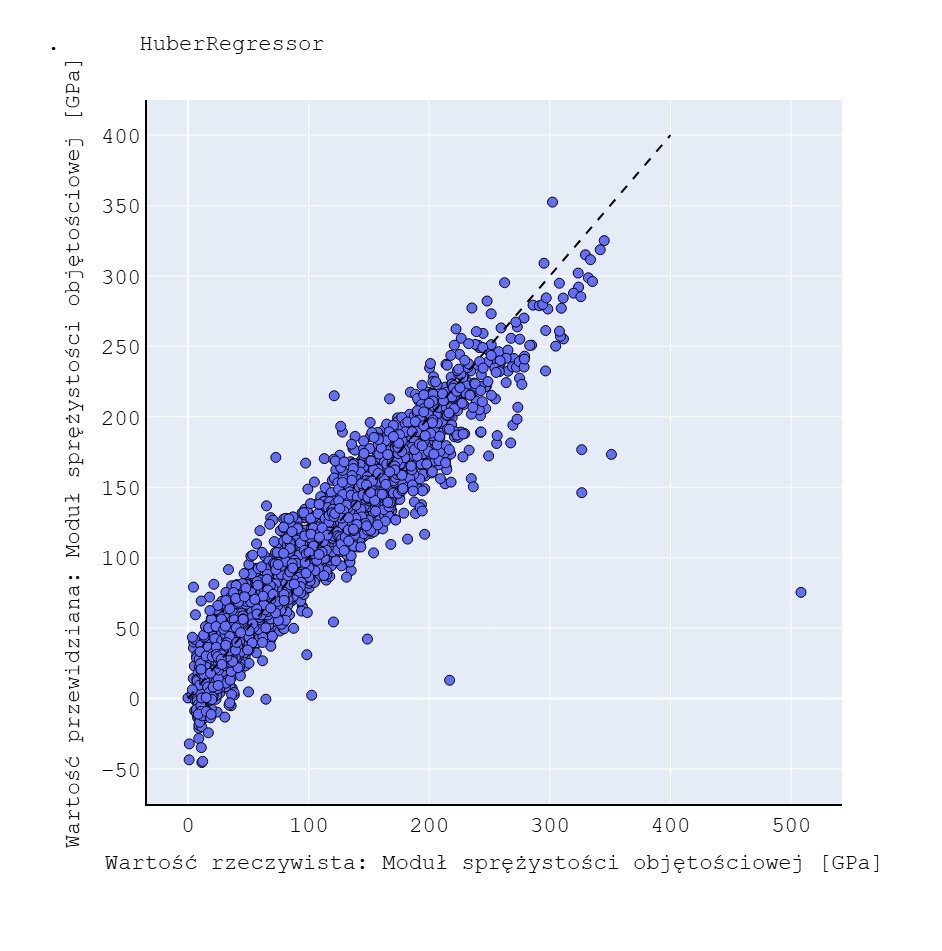
\includegraphics[width=0.48\textwidth]{images/figures/newplot (4).png}
}
\subfigure[Moduł sprężystości poprzecznej]{%
    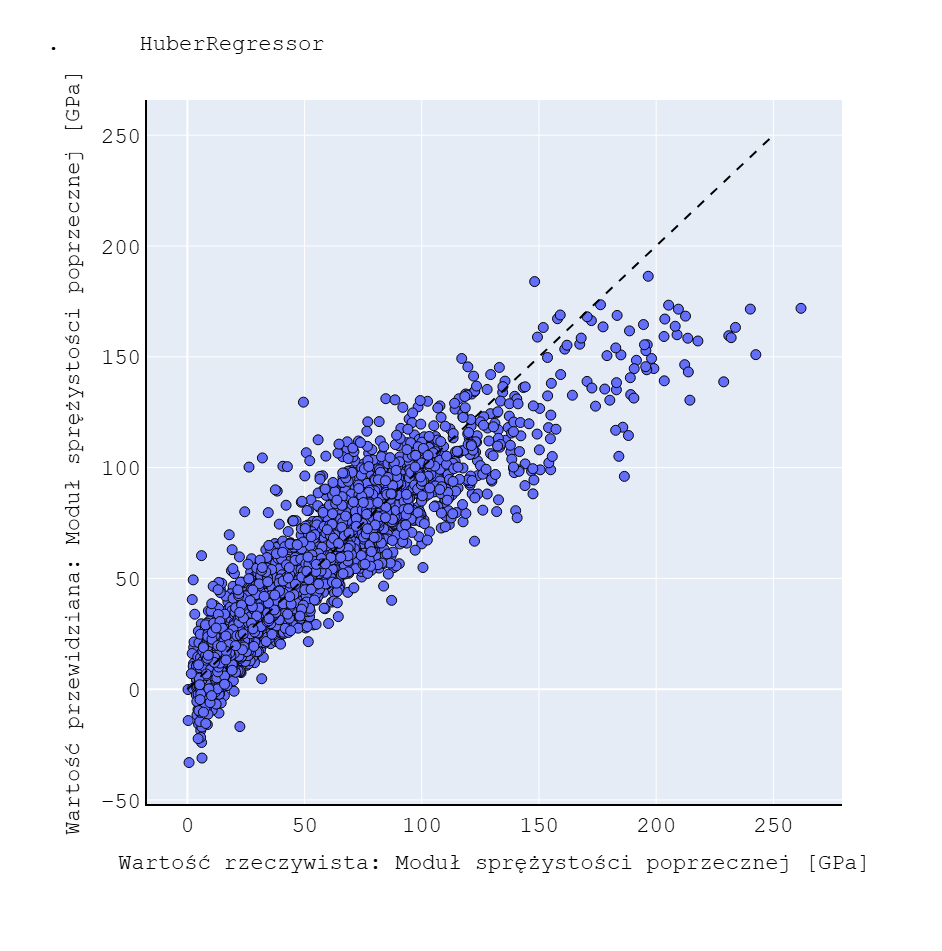
\includegraphics[width=0.48\textwidth]{images/figures/newplot (13).png}
}
\\
\subfigure[Współczynninik Anizotropii]{%
    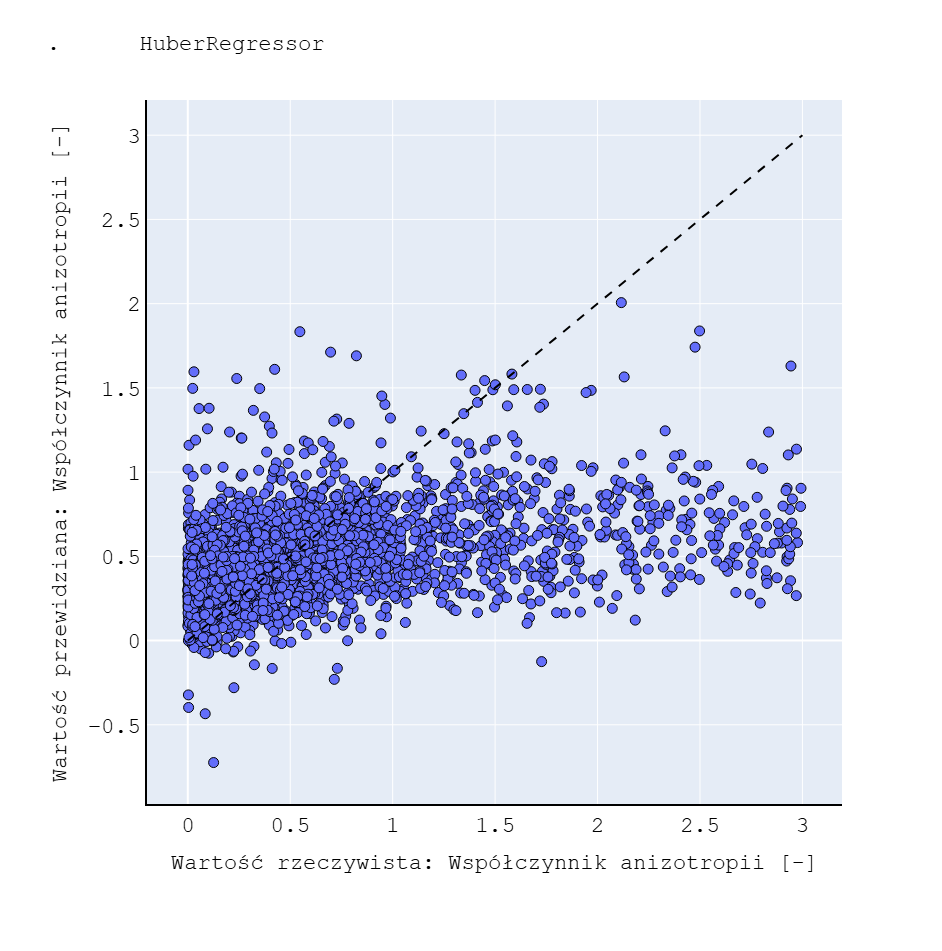
\includegraphics[width=0.48\textwidth]{images/figures/newplot (22).png}
}
\subfigure[Liczba Poisona]{%
    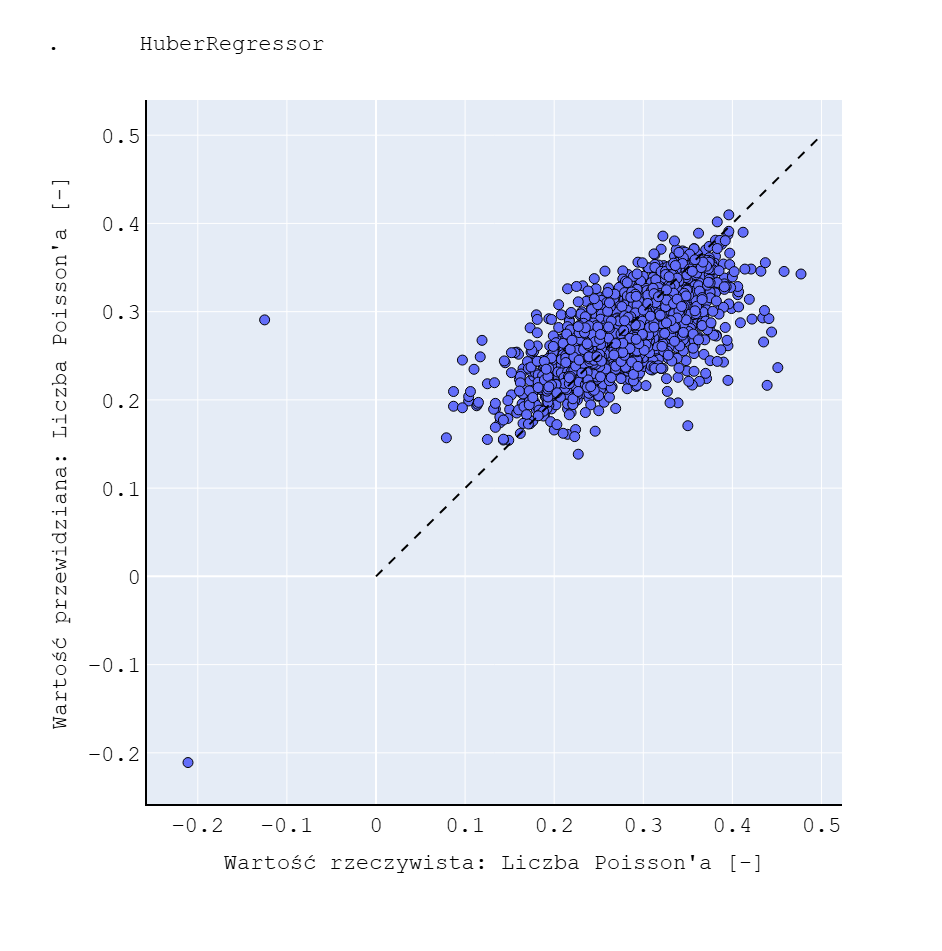
\includegraphics[width=0.48\textwidth]{images/figures/newplot (31).png}
}
\caption{Regresja Huber'a}
\end{figure}


podsumowanie liniowych

\clearpage
\begin{figure}[ht]
\centering
\subfigure[Moduł sprężystości objętościowej]{%
    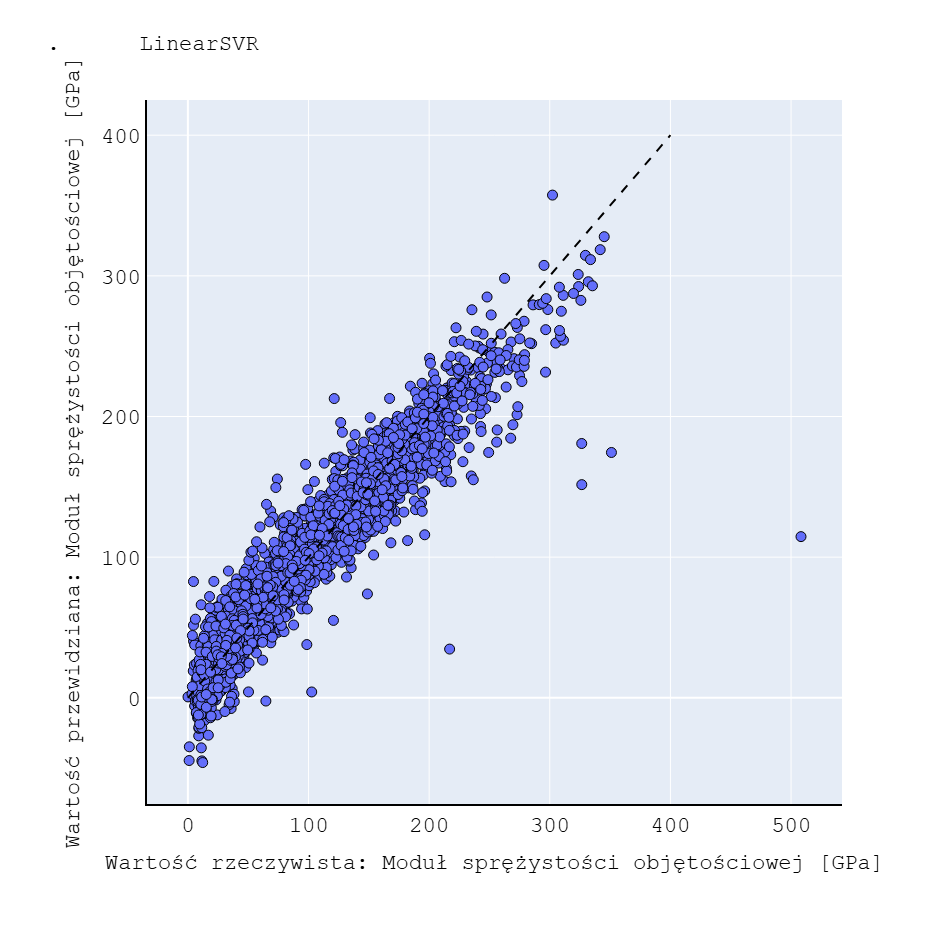
\includegraphics[width=0.48\textwidth]{images/figures/newplot (5).png}
}
\subfigure[Moduł sprężystości poprzecznej]{%
    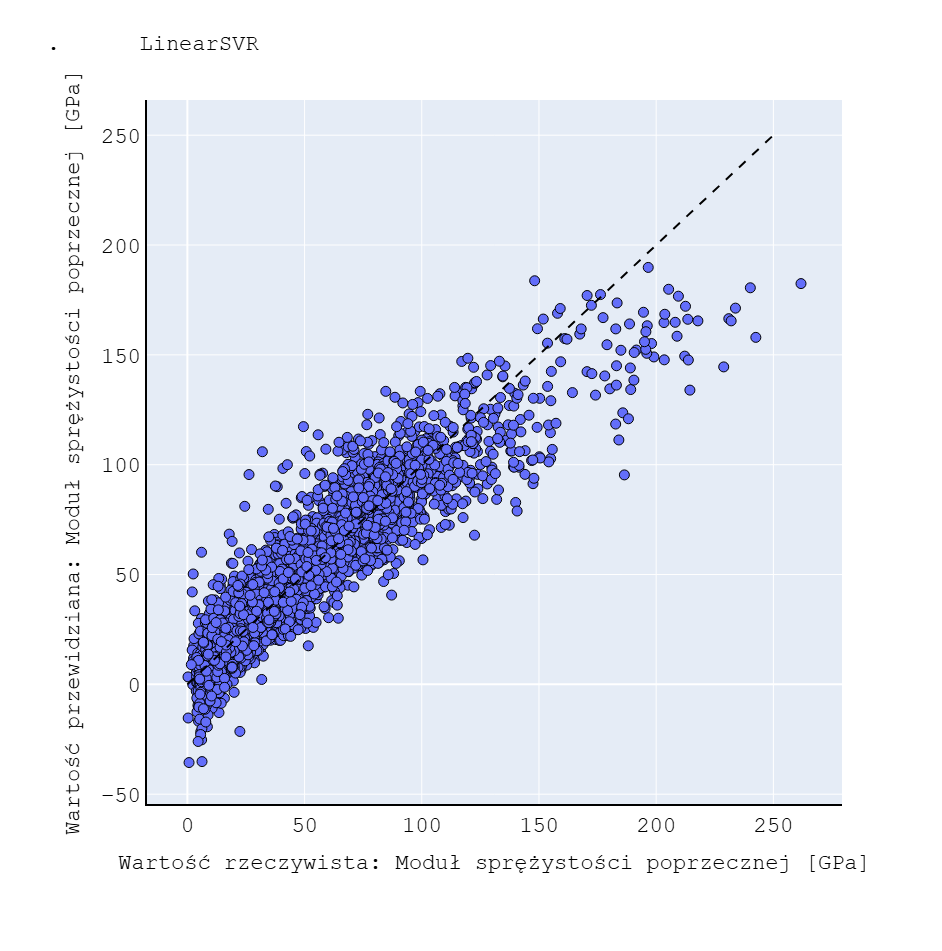
\includegraphics[width=0.48\textwidth]{images/figures/newplot (14).png}
}
\\
\subfigure[Współczynninik Anizotropii]{%
    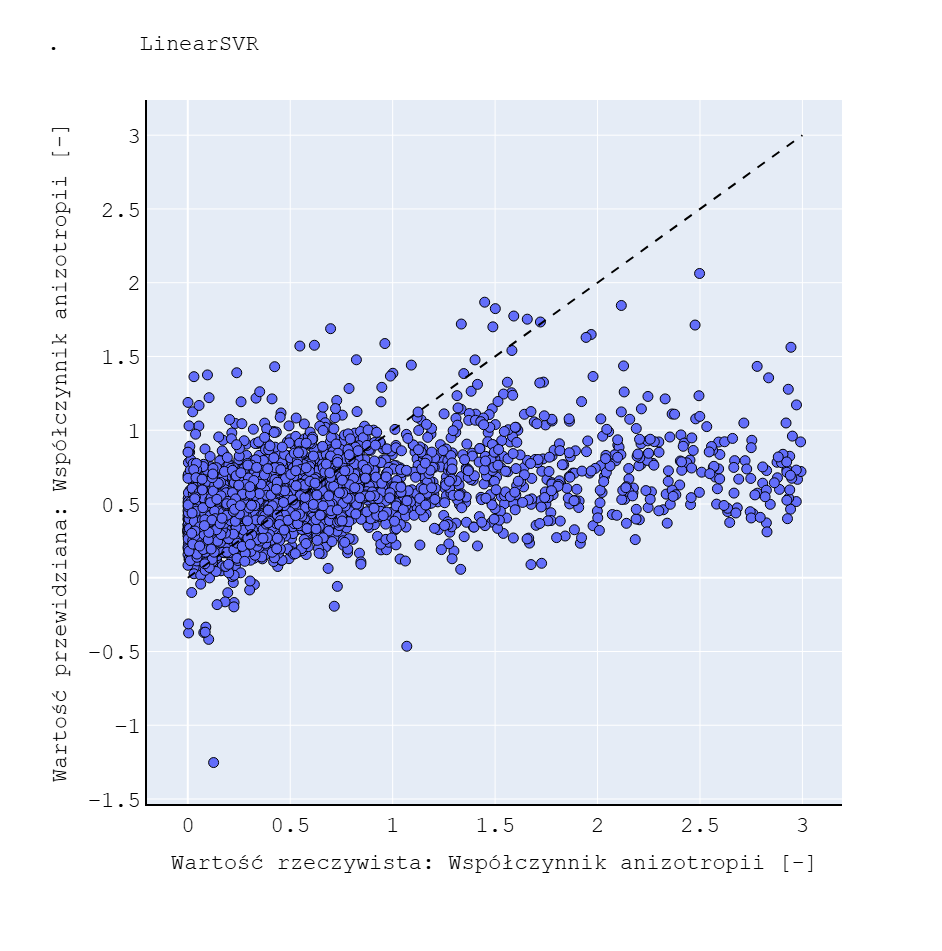
\includegraphics[width=0.48\textwidth]{images/figures/newplot (23).png}
}
\subfigure[Liczba Poisona]{%
    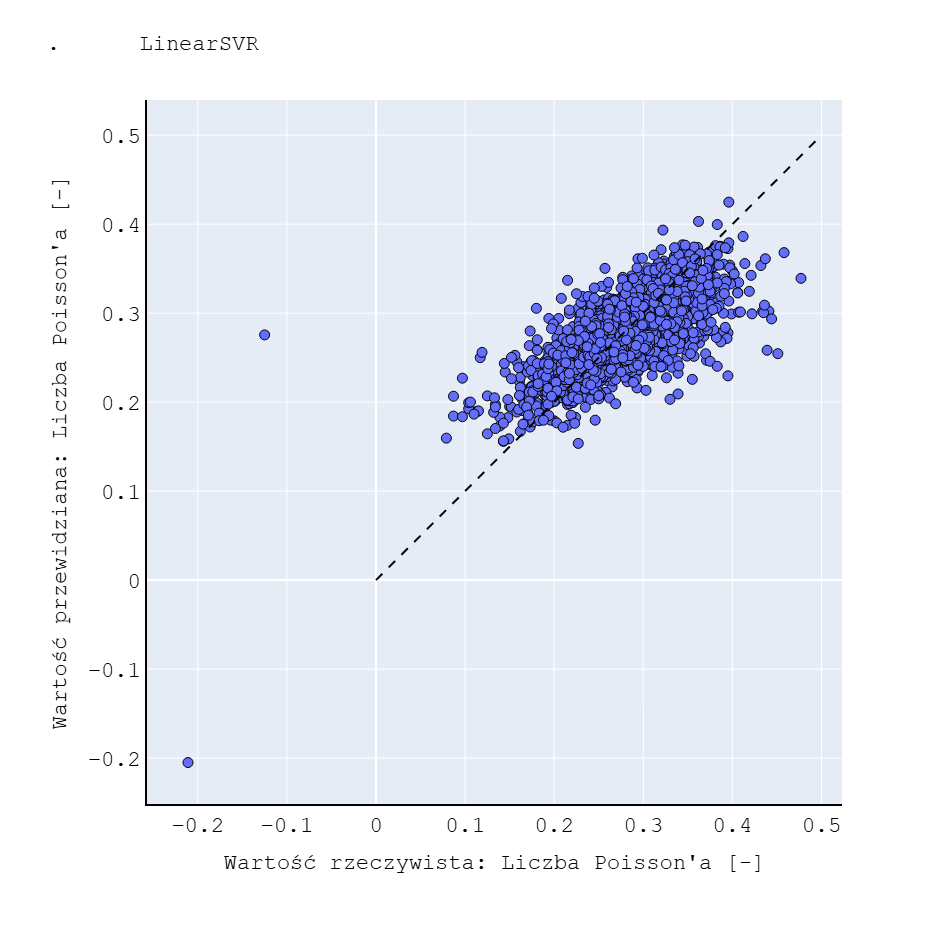
\includegraphics[width=0.48\textwidth]{images/figures/newplot (32).png}
}
\caption{Regresja liniowego SVR}
\end{figure}



\clearpage
\begin{figure}[ht]
\centering
\subfigure[Moduł sprężystości objętościowej]{%
    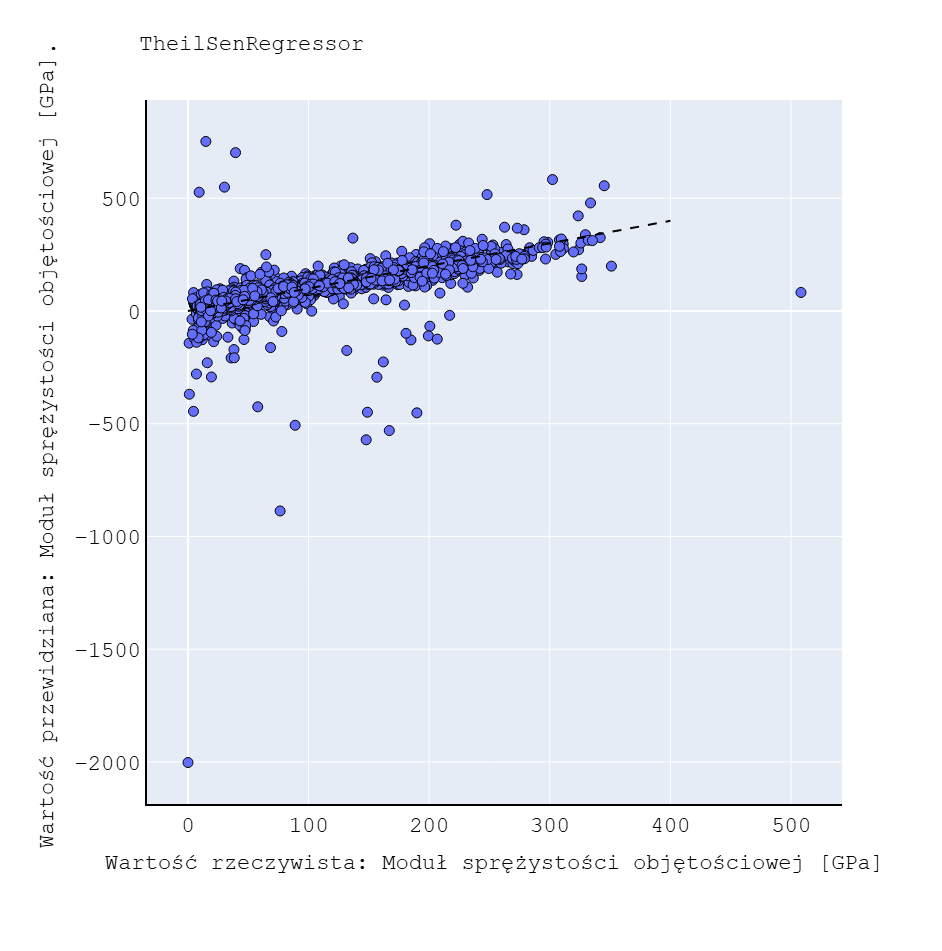
\includegraphics[width=0.48\textwidth]{images/figures/newplot (6).png}
}
\subfigure[Moduł sprężystości poprzecznej]{%
    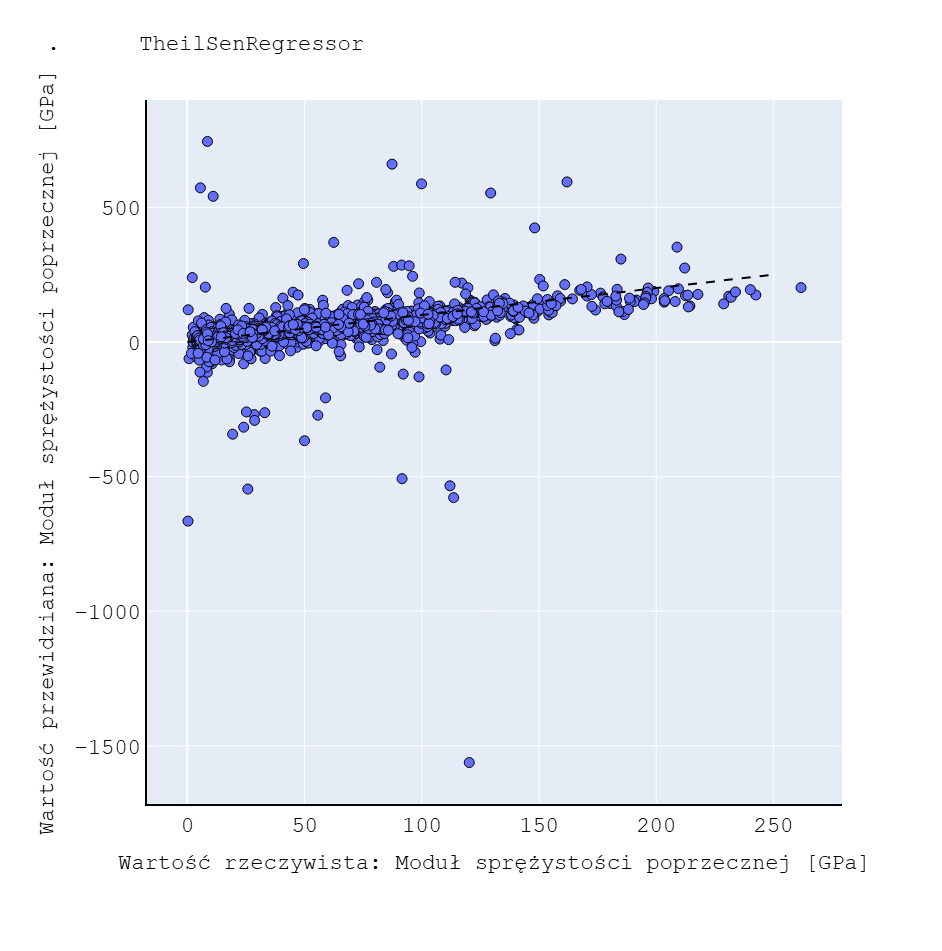
\includegraphics[width=0.48\textwidth]{images/figures/newplot (15).png}
}
\\
\subfigure[Współczynninik Anizotropii]{%
    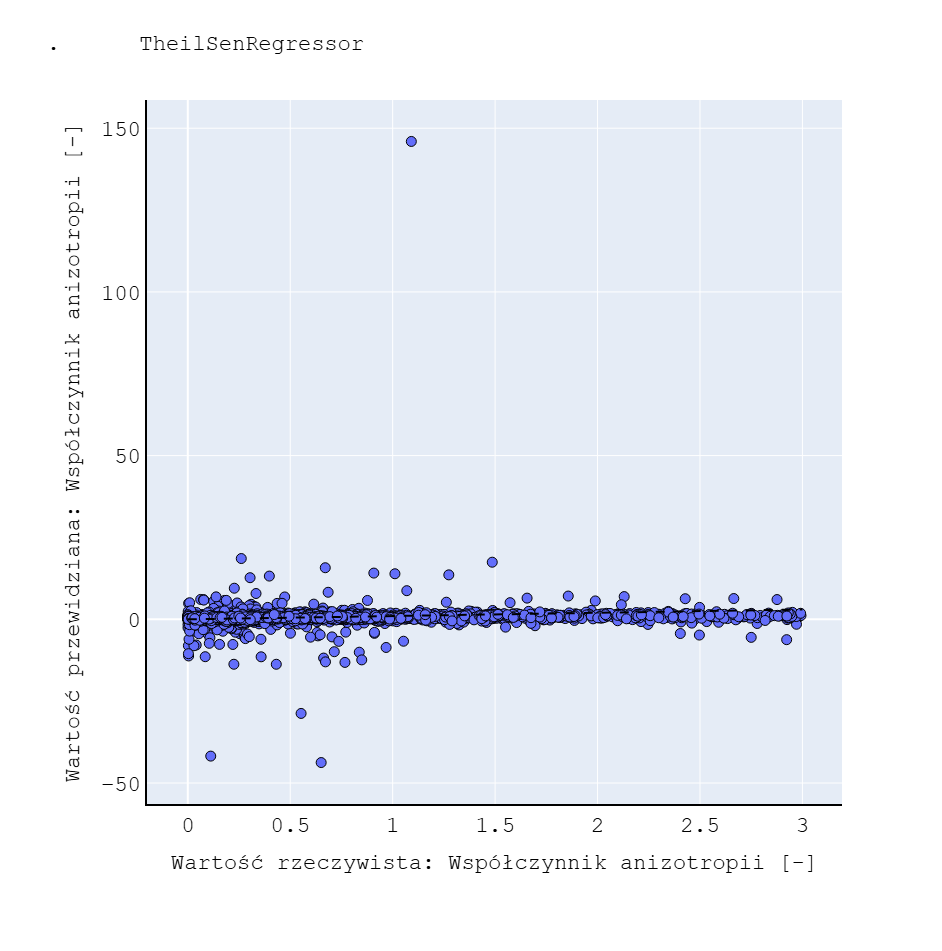
\includegraphics[width=0.48\textwidth]{images/figures/newplot (24).png}
}
\subfigure[Liczba Poisona]{%
    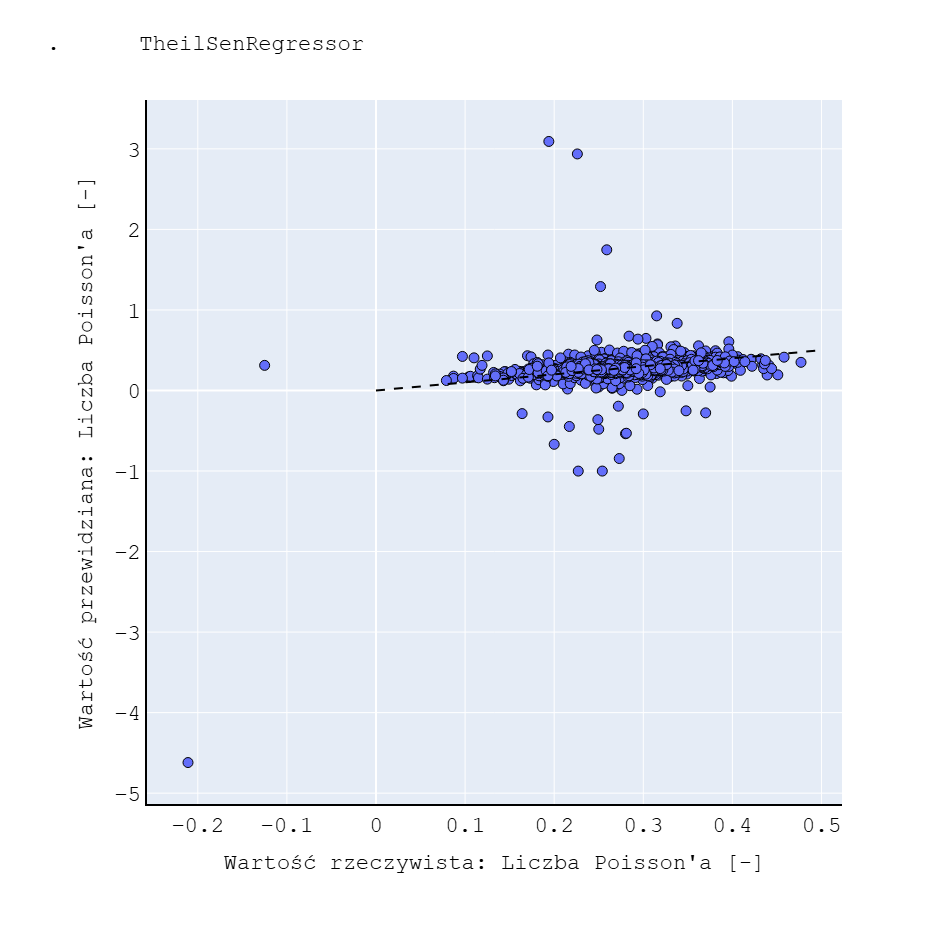
\includegraphics[width=0.48\textwidth]{images/figures/newplot (33).png}
}
\caption{Regresja Theil-Sen}
\end{figure}


opis
\clearpage
\begin{figure}[ht]
\centering
\subfigure[Moduł sprężystości objętościowej]{%
    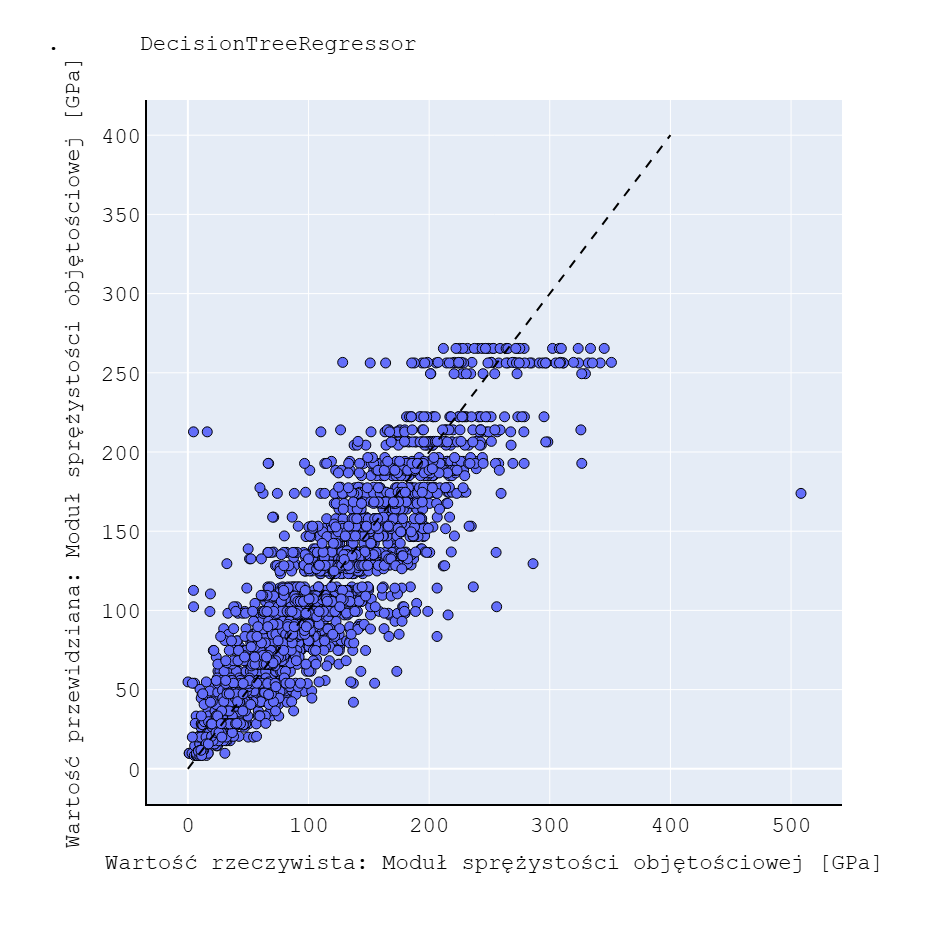
\includegraphics[width=0.48\textwidth]{images/figures/newplot (7).png}
}
\subfigure[Moduł sprężystości poprzecznej]{%
    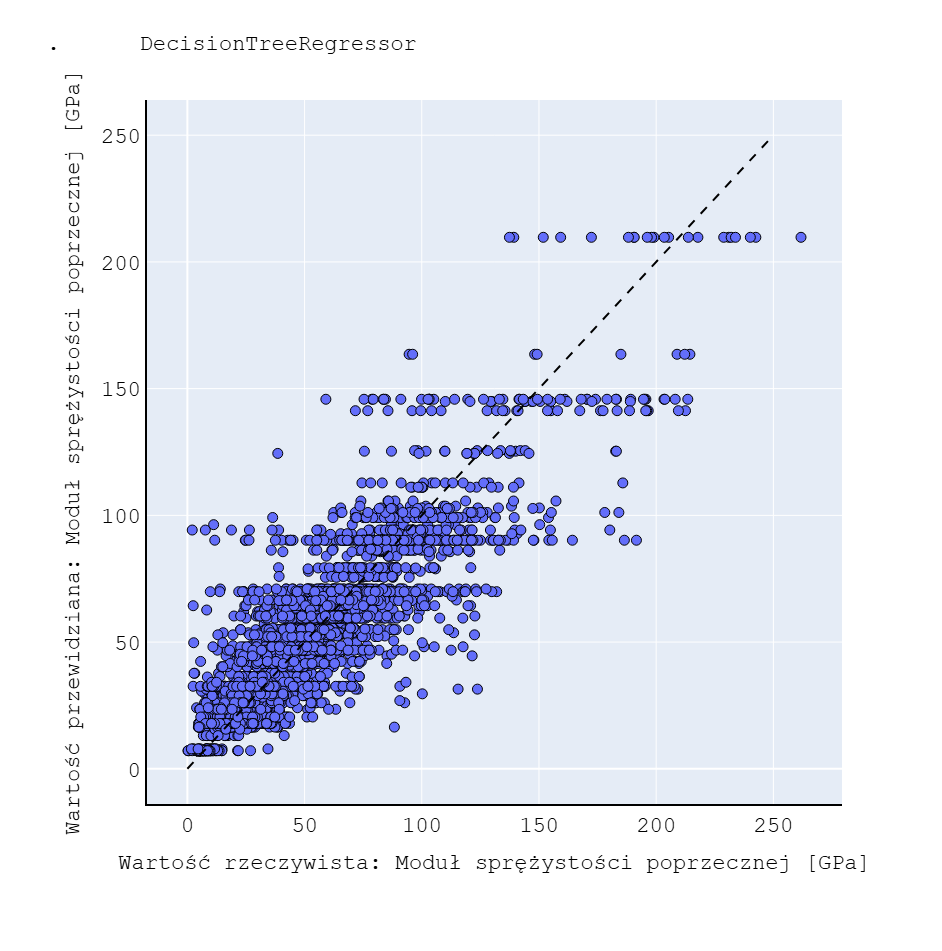
\includegraphics[width=0.48\textwidth]{images/figures/newplot (16).png}
}
\\
\subfigure[Współczynninik Anizotropii]{%
    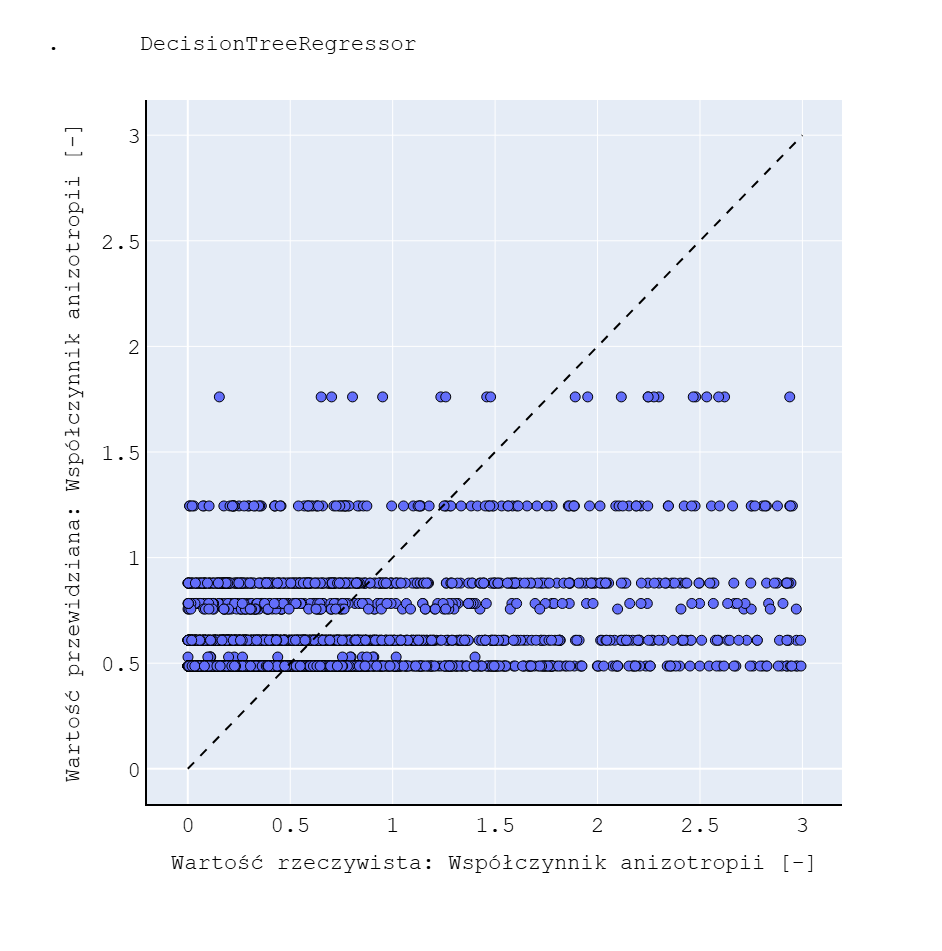
\includegraphics[width=0.48\textwidth]{images/figures/newplot (25).png}
}
\subfigure[Liczba Poisona]{%
    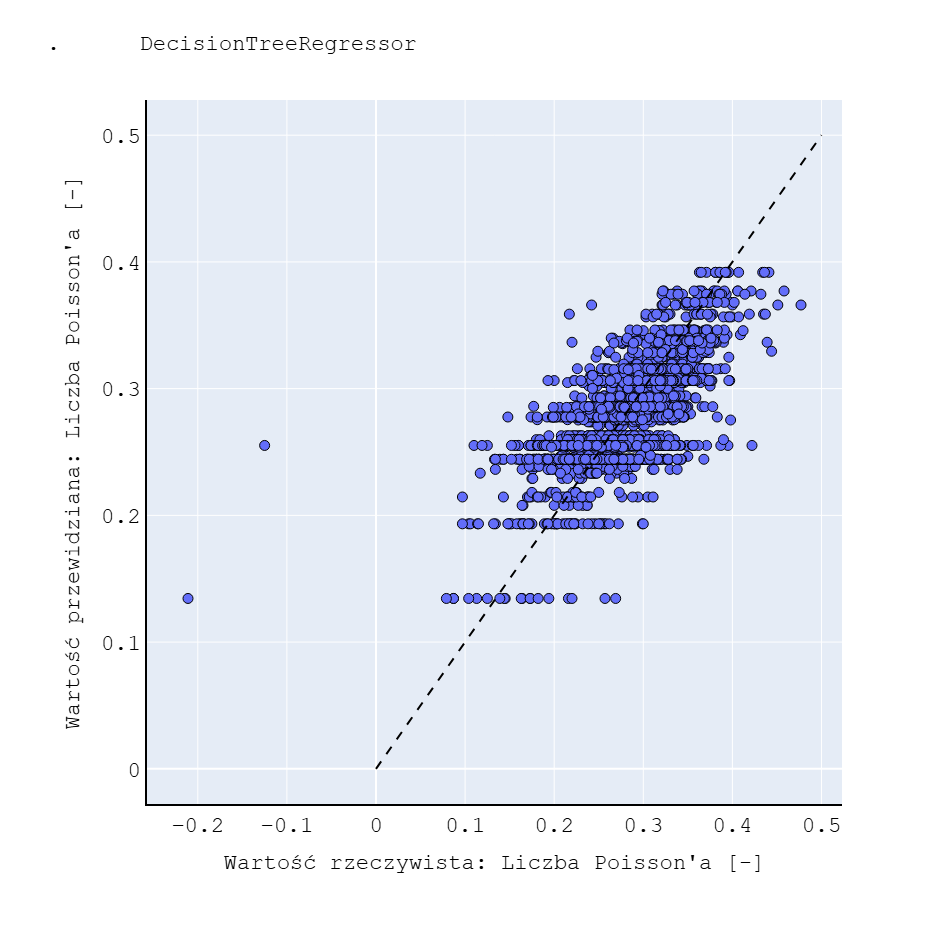
\includegraphics[width=0.48\textwidth]{images/figures/newplot (34).png}
}
\caption{Regresor Drzewa Decyzyjnego}
\end{figure}

\clearpage
\begin{figure}[ht]
\centering
\subfigure[Moduł sprężystości objętościowej]{%
    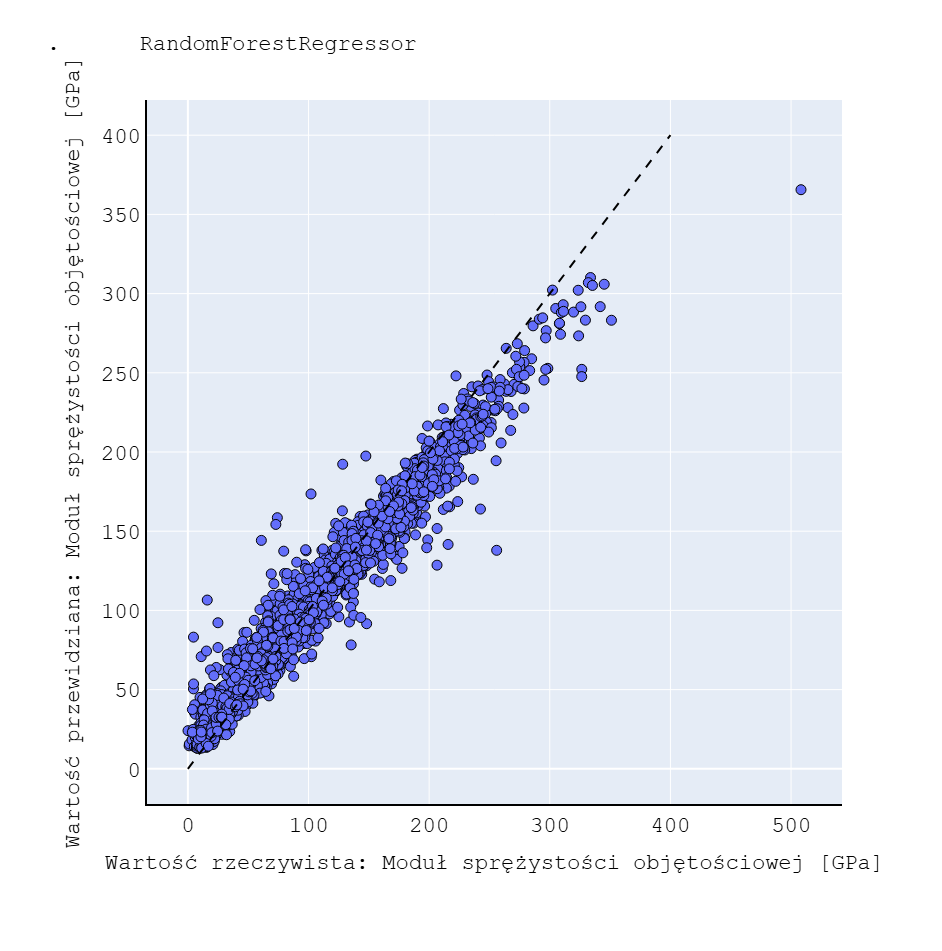
\includegraphics[width=0.48\textwidth]{images/figures/newplot (8).png}
}
\subfigure[Moduł sprężystości poprzecznej]{%
    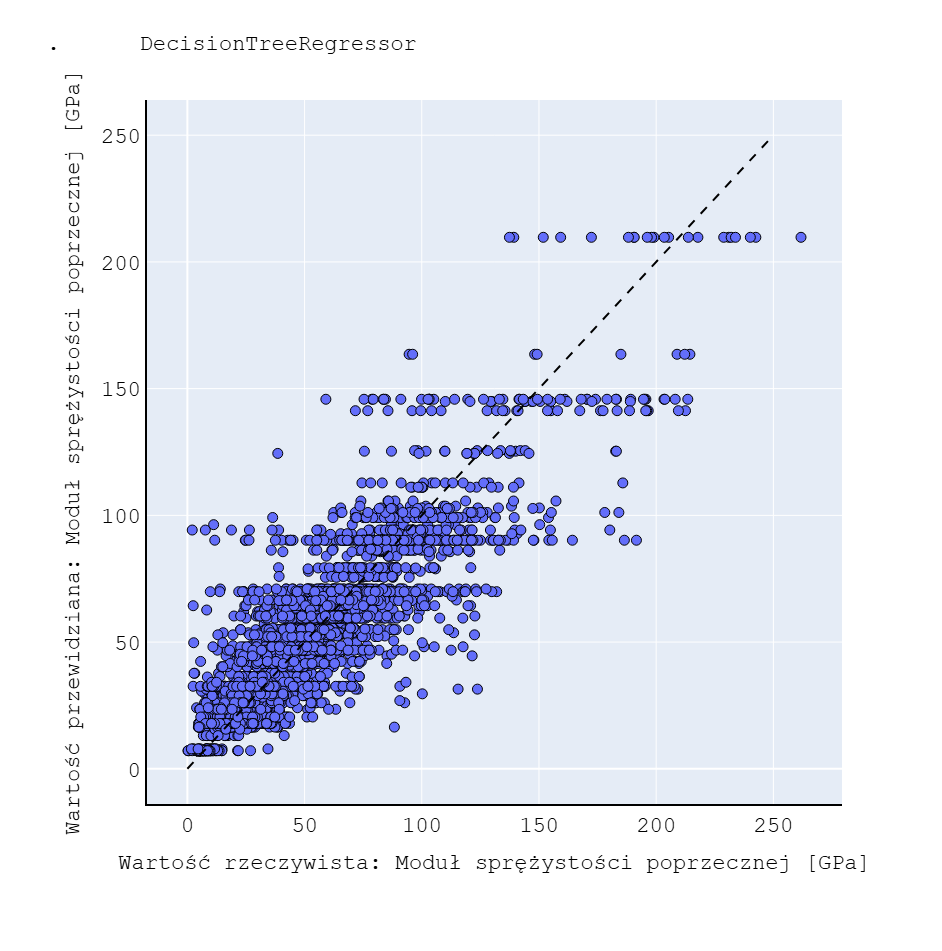
\includegraphics[width=0.48\textwidth]{images/figures/newplot (16).png}
}
\\
\subfigure[Współczynninik Anizotropii]{%
    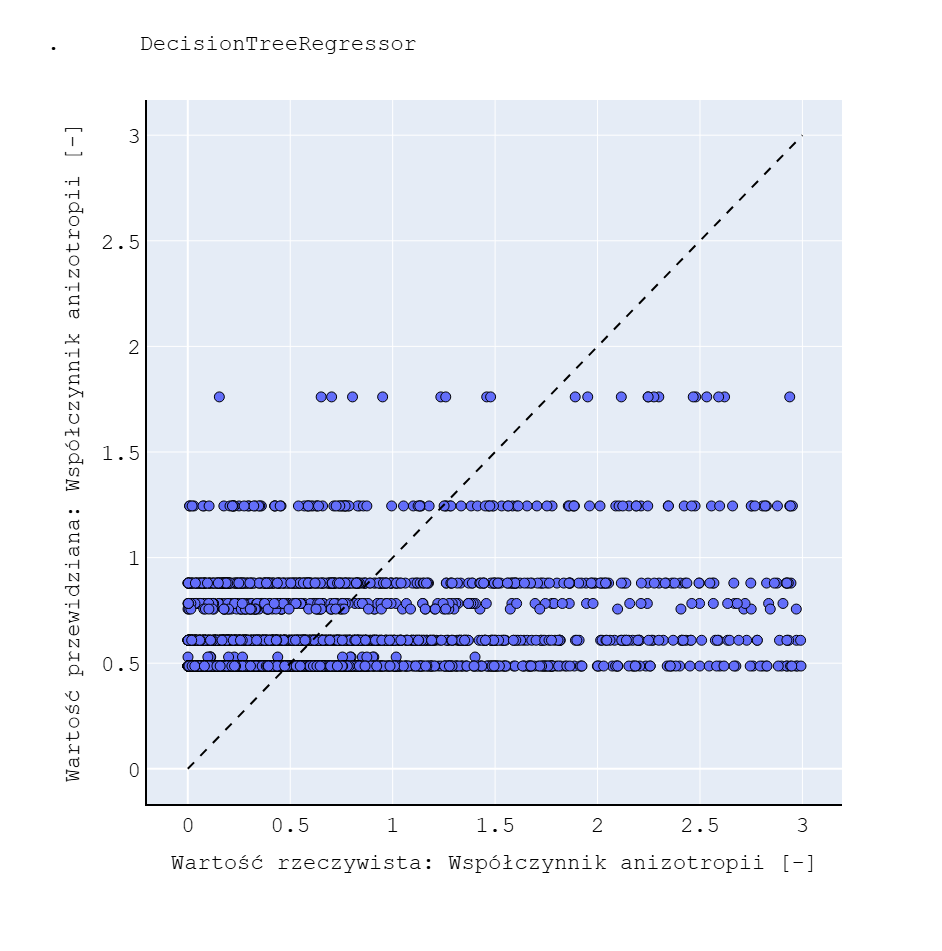
\includegraphics[width=0.48\textwidth]{images/figures/newplot (25).png}
}
\subfigure[Liczba Poisona]{%
    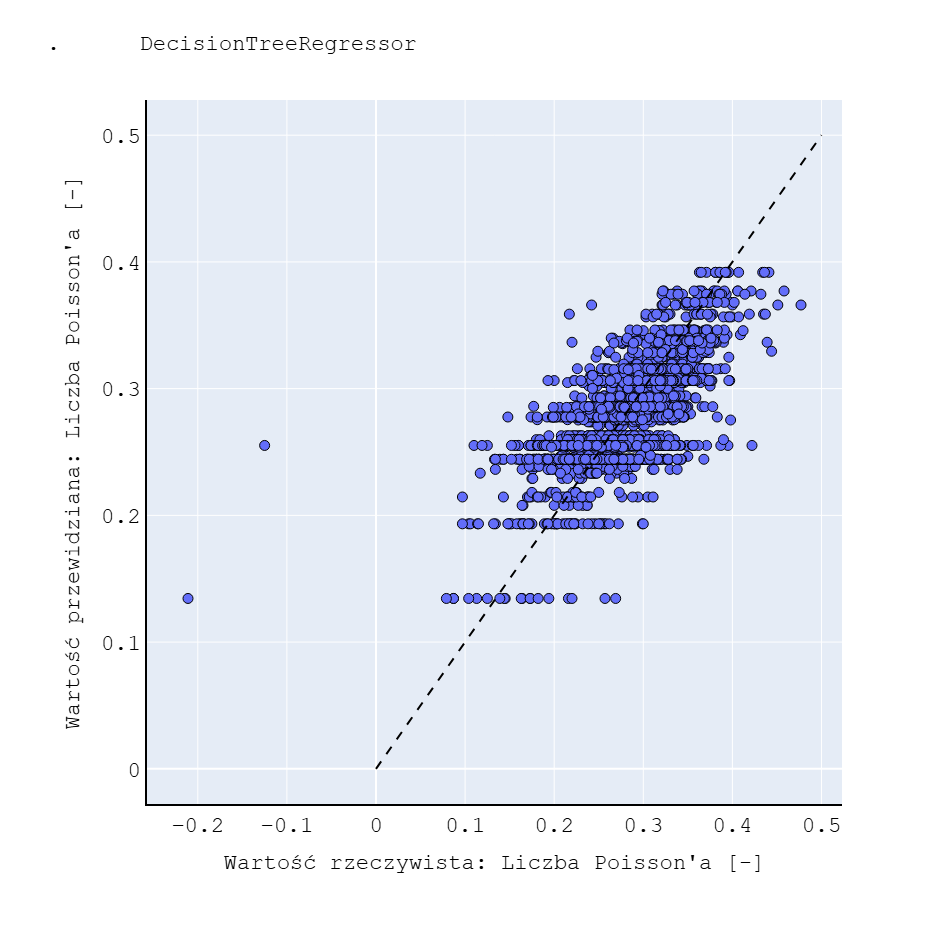
\includegraphics[width=0.48\textwidth]{images/figures/newplot (34).png}
}
\caption{Regresor Losowego Lasu}
\end{figure}



% \clearpage



\begin{tabular}{llrrr}
\toprule
 &  & r2 & rmse & time_taken \\
feature & model &  &  &  \\
\midrule
\multirow[t]{9}{*}{bulk_modulus} & LinearRegression & 0.909000 & 18.787000 & 0.100000 \\
 & Lasso & 0.910000 & 18.756000 & 0.080000 \\
 & Ridge & 0.910000 & 18.753000 & 1.150000 \\
 & ElasticNet & 0.911000 & 18.627000 & 1.030000 \\
 & HuberRegressor & 0.910000 & 18.748000 & 2.230000 \\
 & LinearSVR & 0.909000 & 18.776000 & 5.320000 \\
 & TheilSenRegressor & 0.408000 & 48.010000 & 6.060000 \\
 & DecisionTreeRegressor & 0.551000 & 41.814000 & 3.990000 \\
 & RandomForestRegressor & 0.822000 & 26.330000 & 98.590000 \\
\cline{1-5}
\multirow[t]{9}{*}{shear_modulus} & LinearRegression & 0.830000 & 15.766000 & 0.020000 \\
 & Lasso & 0.834000 & 15.587000 & 0.070000 \\
 & Ridge & 0.831000 & 15.733000 & 1.050000 \\
 & ElasticNet & 0.835000 & 15.556000 & 1.110000 \\
 & HuberRegressor & 0.833000 & 15.633000 & 2.040000 \\
 & LinearSVR & 0.827000 & 15.906000 & 11.110000 \\
 & TheilSenRegressor & 0.005000 & 38.184000 & 6.800000 \\
 & DecisionTreeRegressor & 0.545000 & 25.824000 & 5.870000 \\
 & RandomForestRegressor & 0.800000 & 17.107000 & 101.640000 \\
\cline{1-5}
\multirow[t]{9}{*}{universal_anisotropy} & LinearRegression & 0.082000 & 0.650000 & 0.020000 \\
 & Lasso & 0.140000 & 0.629000 & 0.060000 \\
 & Ridge & 0.109000 & 0.640000 & 1.680000 \\
 & ElasticNet & 0.146000 & 0.627000 & 0.860000 \\
 & HuberRegressor & 0.062000 & 0.657000 & 2.100000 \\
 & LinearSVR & 0.068000 & 0.655000 & 72.390000 \\
 & TheilSenRegressor & -3.139000 & 1.380000 & 3.590000 \\
 & DecisionTreeRegressor & 0.045000 & 0.663000 & 3.960000 \\
 & RandomForestRegressor & 0.180000 & 0.614000 & 96.480000 \\
\cline{1-5}
\multirow[t]{9}{*}{homogeneous_poisson} & LinearRegression & 0.492000 & 0.036000 & 0.010000 \\
 & Lasso & 0.502000 & 0.035000 & 0.040000 \\
 & Ridge & 0.493000 & 0.036000 & 0.970000 \\
 & ElasticNet & 0.502000 & 0.035000 & 0.440000 \\
 & HuberRegressor & 0.488000 & 0.036000 & 2.230000 \\
 & LinearSVR & 0.493000 & 0.036000 & 25.960000 \\
 & TheilSenRegressor & -2.024000 & 0.087000 & 3.920000 \\
 & DecisionTreeRegressor & 0.264000 & 0.043000 & 3.750000 \\
 & RandomForestRegressor & 0.539000 & 0.034000 & 97.040000 \\
\cline{1-5}
\bottomrule
\end{tabular}


\clearpage
